\section{Introduction}
As the AI goes further in its evolution, together with explosion of interconnected IoT devices, the need to move the computation to the "edge" gets more urgent. Wereable devices relying on AI algorithms (such as neural networks) most of the times must stream data to general-purpose devices (such as smartphones and laptops) or to cloud services. The fact that, in real-time applications this represents a serious issue, is known, as well as the numerous legal concerns regarding data manipulation and privacy. All these problems get more mitigated as data and computation are kept local. But close to these debats there is a more subtle problem related to scalability. As heterogeneus data sources increase in number, in fact it becomes computationally expensive to scale a cloud-hosted AI application, in such cases is required to process a huge amount of different kinds of information for instance from a wide network of distributed sensor nodes. It may help, in such cases to let small sensing devices to solve simple classification tasks without involving external services, or even think to partition a complex AI task in smaller ones, moving part of the problem to the edge of a large infrastructure. This kind of scenario now are more feasable thanks to new tools such as STM32CubeAI, that speeds up embedded code development involing neural networks. In this study a simple classification problem using embedded neural network will be analyzed in order to highlight which advantages can be obtained by moving AI algorithms on embedded devices 

\subsection{A Possible Scenario}
Let suppose to be in an hospital with several patients with serious pathological conditions or mental illness. In some case a patient is constrained in its movements, he cannot wake up from bed doing particular stressful movements or take specific positions, it may also be  that such movements are symptoms of agitation that requires immediate medical intervention. These kind of patients must be monitored by mean of wereable sensors to detect anomaly conditions. Such system most of the times consists in a centralized architectures based on a AI algorithm processing data acquired from heterogeneous sensors distributed all over the building complex, in charge of classifying the condition of each specific patient. As the number of patients to be observed grows up the need of c

\subsection{Summary of the work}
In this project a possible solution to the above mentioned problem is proposed in sort of toy example that can perfectly represent the potential effects of moving classification tasks on special-purpose embedded platforms. The purpose of the classification task is to recognize a set of movements and positions of the human body by simply using an STM32 Nucleo board. The motivation of this early choice is based on the fact that when dealing with AI in the embedded field, one of the most tricky task for programmers is the implementation of standard aspects related to popular AI algorithms (in case of neural networks: layers, activation functions and so on), sometime is possible to speed-up this long and tedious part of the development process thanks to libraries and tools provided by silicon manufacturers. All the stages from data gathering, through modeling and training the neural network, to the development of the firmware code will be discussed, remarking the advantages of recurring to embedded software tools and APIs directly provided by MCU manufacturing companies. The peculiarity of the study is the simplicity of the process that led from the network model to the embedded code. At this stage most of the work was performed by a powerful plugin integrated into the STM32CubeMX program, STM32Cube.AI realized by ST Microelectronics to facilitate bare-metal development. Another important result of this work is that the generated network code has been deployed directly on top of a real-time operating system, Miosix, showing the benefits of exploiting typical characteristics of this OS in the field of edge AI.   
\pagebreak

\section{Design and implementation}
It may help to have an high-level view of all the steps of the development process before starting to describe in detail:\\
\begin{wrapfigure}{r}{0.5\textwidth}
	\begin{center}
		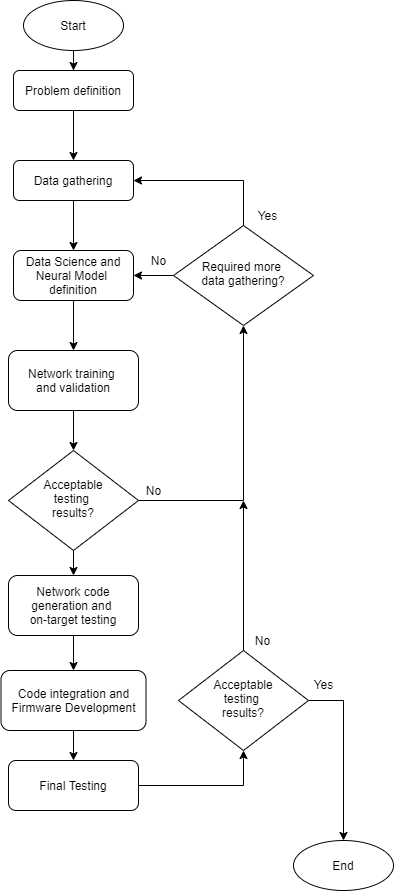
\includegraphics[scale=0.6]{figures/design_steps.png}
		\caption{Design Process Chart}
	\end{center}
\centering
\vspace{-90pt}
\end{wrapfigure}
\begin{itemize}
	\item \textbf{Problem Definition}: discussion about the topic of the project, identification of candidate sensors for data collection, first strategy of the design process and framework to be used for the AI part.
	\item \textbf{Data Gathering}: after being provided with all the required hardware set, development of a basic set of drivers and a firmware for data collection
	\item \textbf{Data Science and Network modeling}: writing and testing of a set of python scripts to manage dataset files, study collected data by computing and plotting some statistics and define a first architecture of the neural network.
	\item \textbf{Network Training and Validation}: training and testing the network iteratively by changing settings, possibly defining new network models, or collecting new data sequence if required, until acceptable performance result is achieved.
	\item \textbf{Network Code Generation and on-target Testing}: set-up of the ST tool STM32CubeAI within STM32CubeMX environment, providing the model obtained in the previous step, performing validation on desktop and on target (on the board) and generate the C code of the input model.
	\item \textbf{Code Integration and Firmware Development}: integration of the output code within the Miosix environment, development of preprocessing routines (if required) and all the other aspects of the final firmware.
	\item \textbf{Final Testing}: testing of the embedded neural network by performing real-time collection and classification of single batches of data samples. 
\end{itemize}
\newpage

\subsection{Problem Definition}
The obviousness of this first step should not mislead from its purpose, as well-known the design cost related to possible errors at first steps is unavoidably amplified through all the subsequent ones. Beyond this observation, some key decisions at this step were taken by looking ahead to the data gathering stage and estimating the possible data demand of the AI algorithm. Classifying movements and positions of the human body is a task that lives naturally in the time domain, so is crucial to understand in detail the phenomenon to be observed and which type of information to be gathered.\newline
There are many ways to measure movements and positions, \textit{inertial} sensors such as the \textit{accelerometer} and \textit{gyroscope} are well-established solutions. \textit{Magnetic} sensors (e.g:\textit{magnetometers}) can also help in capturing motion patterns if used in combination with accelerometers and gyroscopes. Some research work in fact, adopt this approach to detect position and orientation of body parts by using sensor fusion techniques \cite{navamelendez2016} and the patterns to be extracted from data are strongly shaped by this information. The problem in this case, is more abstract and requires a considerable amount of data to be collected, from many sources, to obtain accurate classification results. This observation is then accentuated considering the cost in terms of time and efforts required to perform data gathering, neural networks as well-known are "data hungry" and regardless their effectivness, no acceptable results can be achieved without a rich dataset. \newline

\subsection{Data Gathering}
This part is strongly affected by some a priori design decision. As stated before this work relies on the STM32CubeAI plugin to speed-up the process that allows to obtain the initializing firmware code of the neural network from some framework-generated model, so only STM32-family hardware is used. After a deep analysis of topic-related studies it has been decided to use a single sensing device located at inguinal level (right-side). This location revealed to be extremely useful for two reasons:
\begin{itemize}
	\item Allows the sensors to detect directional and angular accelerations of the right lower limb which characterizes most of the movements and positions that must be classified 
	\item Avoid the person wearing the device to be hampered during activity sessions
\end{itemize}
From hardware perspective, a first evaluation of the model complexity and resource avalability suggested two different solutions:
\begin{itemize}
	\item NUCLEO-F401RE: a prototyping board based on a STM32-family MCU, the F401RE (ARM Cortex M4).
	\item IKS01A2 Sensor board, equipped with 3 inertial sensors (LSM6DSL 3D Accelerometer and 3D Gyroscope and LSM303AGR 3D Accelerometer), 1 magnetic sensor (LSM303AGR Magnetometer), 1 temperature and humidity sensor (HTS221) and 1 pressure sensor (LPS22HB)
\end{itemize} 
\begin{figure}[H]
	\centering
	\begin{subfigure}[H]{0.45\textwidth}
		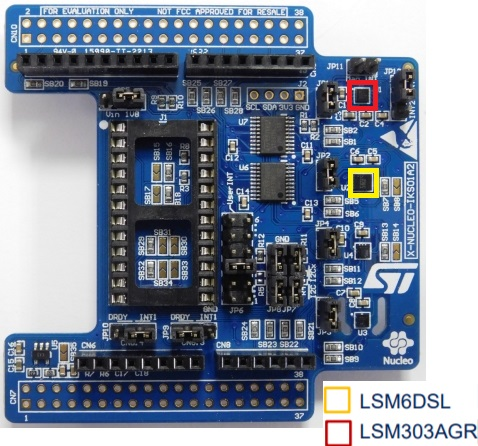
\includegraphics[scale=0.8]{figures/iks01a2.jpg} 
		\caption{IKS01A2 Sensor Board}\label{fig:2a}
	\end{subfigure}
	\hfill
	\begin{subfigure}[H]{0.45\textwidth}
		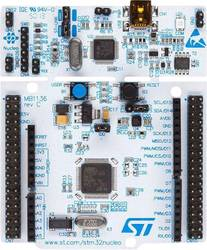
\includegraphics[scale=0.8]{figures/stm32f401re.jpg} 
		\caption{STM32F401RE Board}\label{fig:2b}
	\end{subfigure}
\end{figure}
A first problem to be solved at this stage consists in finding a feasable way to store sensor-collected information.\newline
Unfortunately it is not possible to use memories on board. On the other hand, the intuitive solution of streaming data samples being directly connected to the laptop through the USB port, is unfeasable because of ambient and cable size constraints. Although Miosix provides support to manage a filesystem on an external SD card, this possibility has been discarded due to the unavailability of a proper board expansion. This forced at the beginning to consider an Arduino MKR1000 board as a WiFi shield to stream data to a laptop using a smartphone as hotspot, but attempts to transfer data from the Nucleo board to the MKR1000 using I2C met some problems and discouraged this approach. In any case the increasing size of the packed boards make them uncomfortable to be worn.\newline
A final and simple solution to the mentioned problems relies on a simple Raspberry Pi Model 3 besides the sensor board:
\begin{center}
	\begin{figure}[H]
		\begin{subfigure}[H]{0.45\textwidth}
			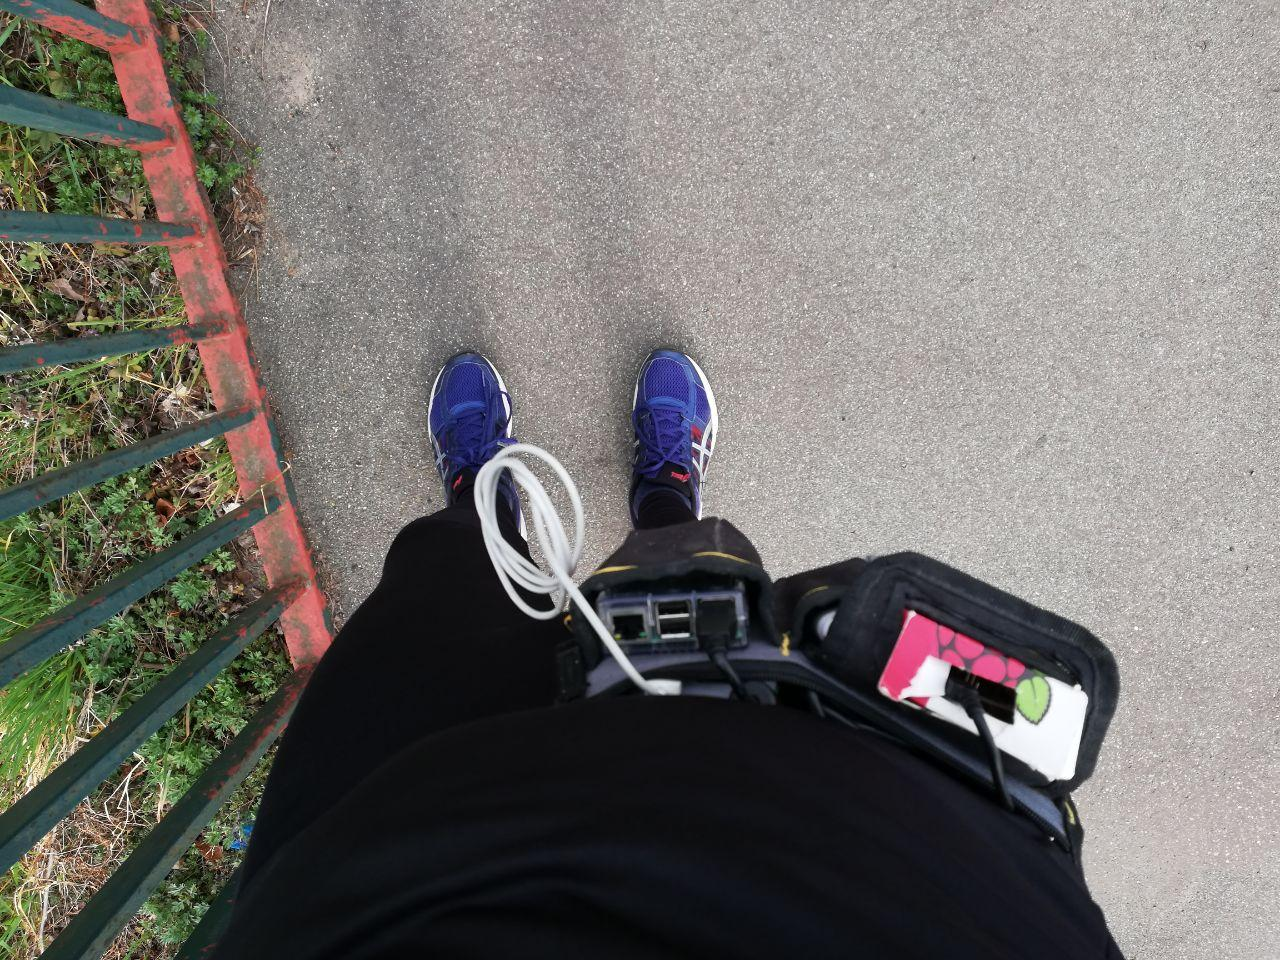
\includegraphics[scale=0.35]{figures/data_gathering_1.jpg}
			\caption{Data gathering activity}\label{fig:3a}
		\end{subfigure}
		\hfill
		\begin{subfigure}[H]{0.45\textwidth}
			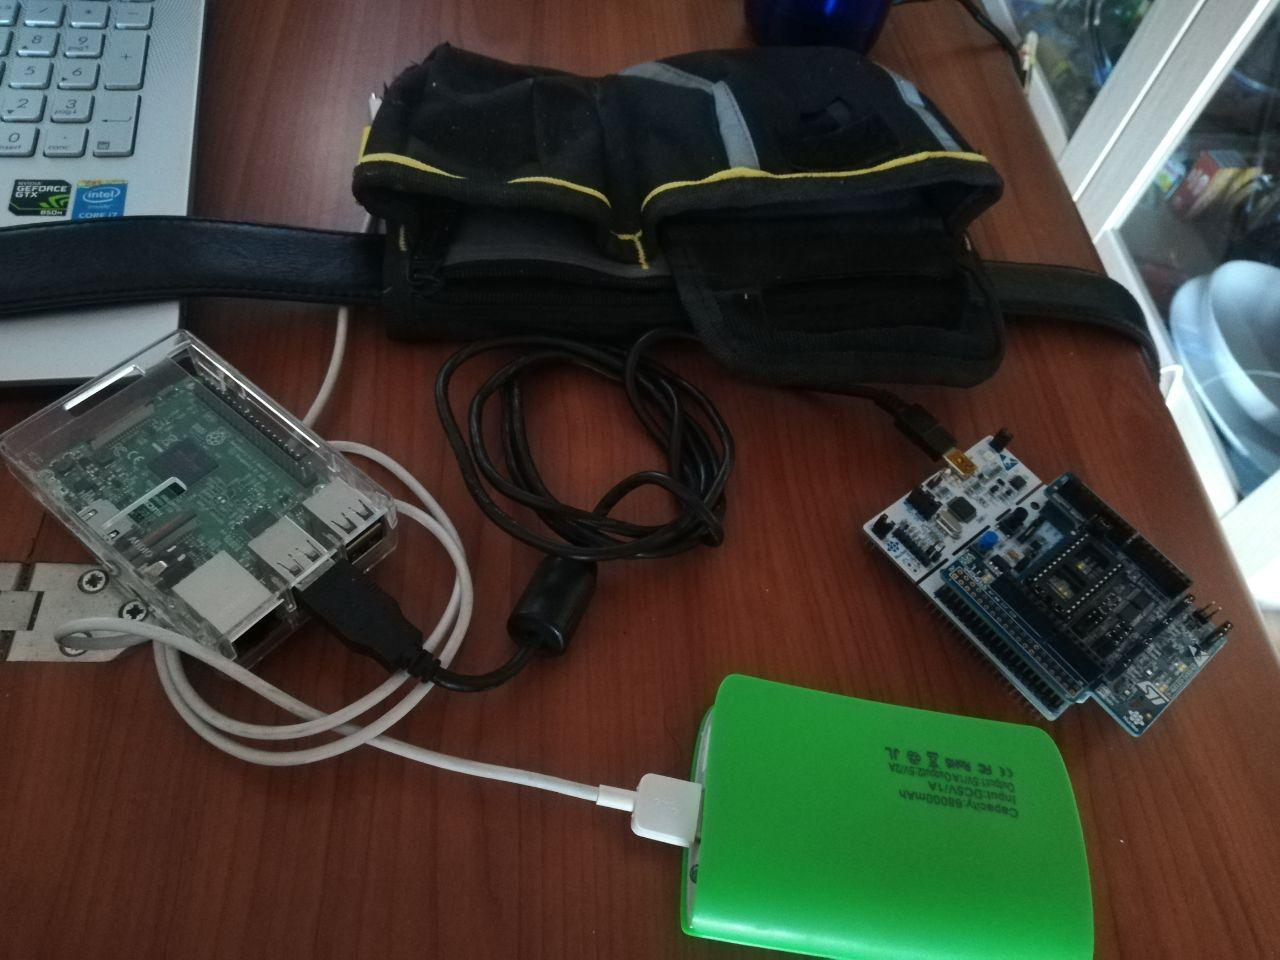
\includegraphics[scale=0.35]{figures/data_gathering_2.jpg}
			\caption{used devices}\label{fig:3b}
		\end{subfigure}
	\end{figure} 
\end{center}
The sensing device streams data in form of comma-separated values that are stored by the Raspberry into a file, while a simple python program on backend is in charge of creating and managing all the activity session files during data collection.\newline
The implementation of such script is straightforward, less trivial is the design and implementation of the MEMS drivers considering the fact that 4 different sensors must be used. Because of time constraints at the beginning, an already implemented version of the drivers were used, this to speed up data gathering stage. The following discussion will be focused instead on a version implemented afterwards, not included in the final test. \newline
An initial remark regards the design pattern adopted for this part. Four sensors are splitted into 2 physical SoCs: the LSM6DSL (accelerometer and gyroscope) and the LSM303AGR (accelerometer and magnetometer), so 2 hardware-proxy classes have been realized \mintinline[bgcolor=whitesmoke]{C++}{LSM6DSLAccGyr} and \mintinline[bgcolor=whitesmoke]{C++}{LSM303AGRAccMag}, both implementing methods to setup control registers and read values from on-chip sensors. The expansion board instead communicates with the MCU using I2C. Since Miosix provides a low-level implementation of I2C, this was exploited to realize a class to perform read and write operations from the sensor board registers. Among the possible configurations by which is possible to connected the sensors, the expansion has been set up with a single shared line connected to all the MEMS' of the IKS01A2, the communication steps to read/write one or more bytes, moreover are generally the same (as specified by the protocol), from such specifications the implementation is straightforward:\\

\begin{center}
	\begin{figure}[H]
		\begin{subfigure}[H]{0.45\textwidth}
			\hfill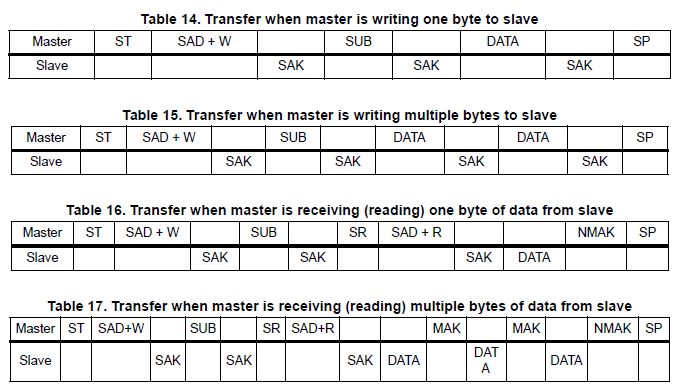
\includegraphics[scale=0.6]{figures/lsm6dsl_datasheet.png}\hspace*{\fill}
			\caption{I2C Communcation}\label{fig:4a}
		\end{subfigure}
		\hfill
		\begin{subfigure}[H]{0.45\textwidth}
			\hfill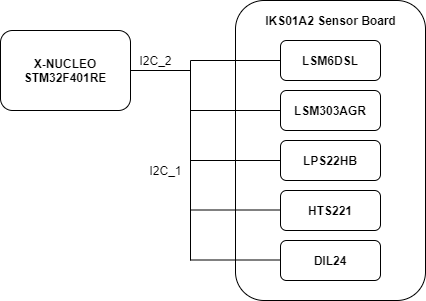
\includegraphics[scale=0.5]{figures/i2c_com.png}\hspace*{\fill}
			\caption{I2C Connection}\label{fig:4b}
		\end{subfigure}
			\begin{subfigure}[H]{0.5\textwidth}
			\inputminted[framesep=1.5cm, firstline=46, lastline=67, bgcolor=whitesmoke, fontsize=\tiny]{C++}{code/i2c_helper.cpp}
			\vspace{-20pt}
			\caption{i2c\_helper.cpp: read}\label{fig:4c}
			\end{subfigure}
		\hfill
		\begin{subfigure}[H]{0.45\textwidth}
			\vspace{+1pt}
			\inputminted[framesep=1.5cm, firstline=90, lastline=112, bgcolor=whitesmoke, fontsize=\tiny]{C++}{code/i2c_helper.cpp}
			\vspace{-20pt}
			\caption{i2c\_helper.cpp: write}\label{fig:4d}
		\end{subfigure}
	\end{figure}
\end{center}

Before proceeding to read data from MEMS, it is required to configure the control registers. Activation and initialization are performed in a single step implemented by the \mintinline[bgcolor=whitesmoke]{C++}{init()} method.\newline

\begin{center}
	\begin{figure}[H]
		\begin{subfigure}[H]{0.5\textwidth}
			\inputminted[framesep=1.5cm, firstline=56, lastline=71, bgcolor=whitesmoke, fontsize=\tiny]{C++}{code/data_gathering.cpp}
			\vspace{-20pt}
			\caption{LSM303AGR.h: io\_read method}\label{fig:5a}
		\end{subfigure}
		\hfill
		\begin{subfigure}[H]{0.5\textwidth}
			\vspace{+1pt}
			\inputminted[framesep=1.5cm, firstline=72, lastline=98, bgcolor=whitesmoke, fontsize=\tiny]{C++}{code/data_gathering.cpp}
			\vspace{-20pt}
			\caption{LSM303AGR.h: io\_write method}\label{fig:5b}
		\end{subfigure}
	\end{figure}
\end{center}
It runs similarly for both LSM6DSL and LSM303AGR, sets default values in those registers that are more likely to be used for data gathering. In both classes, with slight differences, \mintinline[bgcolor=whitesmoke]{C++}{io_read()} and \mintinline[bgcolor=whitesmoke]{C++}{io_write()} act as a I2C interface to allow read and write operation respectively involving device, register addresses and bit masks\newline 
Crucial aspects of sensor configuration are:
\begin{itemize}
	\item \textbf{Output data rate}: representing the frequency at which the device provides new values
	\item \textbf{Full scale value}: the range of values that the sensor can represent, changing the FS, the sensitivity is affected as well.  
	\item \textbf{Sensitivity}: the minimum variation of the quantity to be measured that can be percepted by the MEMS. Sensitivity can also change according to the power mode in which the sensor is used.
\end{itemize}
All these values are set and shown in the initial steps of the program execution, specifically in this work: 



\begin{table}[H]
	\begin{subtable}[H]{0.45\textwidth}
		\begin{tabular}{||p{6cm}|p{2cm}||}
			\hline
			\textbf{LSM6DSL Accelerometer} 	& 				 		\T\B  \\ 
			\hline
			ODR				  				& 	    208 Hz 	 		\T\B  \\
			Full scale						&	    2.0 g 	 		 \T\B  \\
			Sensitivity						& 		0.061	\tiny[mg/LSB]	 \T\B  \\
			\hline
		\end{tabular}
		\vspace{10pt}
	\end{subtable}
	\hfill
	\begin{subtable}[H]{0.45\textwidth}
		\begin{tabular}{||p{6cm}|p{2cm}||}
			\hline
			\textbf{LSM6DSL Gyroscpe} 	& 				 	 				 \T\B  \\ 
			\hline
			ODR				  				& 	    208 Hz 	 				 \T\B  \\
			Full scale						&	    2000 dps 				 \T\B  \\
			Sensitivity						& 		70.0 \tiny[mdps/LSB]	 \T\B  \\
			\hline
		\end{tabular}
	\vspace{10pt}
	\end{subtable}

	\begin{subtable}[H]{0.45\textwidth}
		\begin{tabular}{||p{6cm}|p{2cm}||}
			\hline
			\textbf{LSM303AGR Accelerometer} 	& 				 \T\B  \\ 
			\hline
			ODR				  				& 	    100 Hz 		 \T\B  \\
			Full scale						&	    2.0 g 	 	 \T\B  \\
			Sensitivity						& 		3.9	\tiny[mg/LSB] 	 \T\B  \\
			\hline
		\end{tabular}
		\vspace{10pt}
	\end{subtable}
	\hfill
	\begin{subtable}[H]{0.45\textwidth}
		\begin{tabular}{||p{6cm}|p{2cm}||}
			\hline 
			\textbf{LSM303AGR Magnetometer} & 				 	 \T\B  \\ 
			\hline
			ODR				  				& 	    100 Hz 	 	 \T\B  \\
			Full scale						&	    49.12 g 	 \T\B  \\
			Sensitivity						& 		1.5	 		 \T\B  \\
			\hline
		\end{tabular}
		\vspace{10pt}
	\end{subtable}
	\centering
	\caption{Data Gathering settings}\label{tab:1}
\end{table}
As it can be noticed, both the accelerometers have been set to the same full scale value, to mantain data coherent with previous datasets already collected, whereas an high value (2000dps) has been chosen for the gyroscope to increase the sensitivity of the MEMS to even small movements of the leg (typical of some positions). In all the cases the configuration can be changed by modifying the \mintinline[bgcolor=whitesmoke]{C++}{IKS01A2_config.h}.\newline
Axes values are read almost the same way for all the sensors, since by design data registers are contiguous a single read scan of 6 bytes (2 byte-value/axis) is performed, raw bytes are then composed and multiplied by the sensitivity. The \mintinline[bgcolor=whitesmoke]{C++}{LSM303AGR::get_acc_axes()} is slightly complex, since it must consider the power mode in which the sensor is used that affects the sensitivity value:
\begin{center}
	\begin{figure}[H]
		\begin{subfigure}[H]{0.5\textwidth}
			\inputminted[framesep=1.5cm, firstline=101, lastline=127, bgcolor=whitesmoke, fontsize=\tiny]{C++}{code/data_gathering.cpp}
			\vspace{-20pt}
			\caption{LSM6DSL.cpp: get\_acc\_axes()}\label{fig:5a}
		\end{subfigure}
		\hfill
		\begin{subfigure}[H]{0.5\textwidth}
			\vspace{+1pt}
			\inputminted[framesep=1.5cm, firstline=149, lastline=189, bgcolor=whitesmoke, fontsize=\tiny]{C++}{code/data_gathering.cpp}
			\vspace{-20pt}
			\caption{LSM303AGR.cpp: get\_acc\_axes()}\label{fig:5b}
		\end{subfigure}
	\end{figure}
\end{center}
 In the implementation of the method \mintinline[bgcolor=whitesmoke]{C++}{LSM303AGR:: get_acc_axes()} the variables \mintinline[bgcolor=whitesmoke]{C++}{a_hr} and \mintinline[bgcolor=whitesmoke]{C++}{a_lp} contain values that encode the resolution and power modes at which the device is used and according to such information a proper shifting is applied to the read values.\newline
 Another interesting aspects of the LSM6DSL (iNEMO) is the maximum ODR the device is able to reach: 1660 Hz. Under strict power requirements, this high rate may represent a problem, fortunately both the sensors offer the possibility to store data in a FIFO  buffer in order to burst all the read values at once and allows the MCU to sleep in the meanwhile. Since the low output data rate, this possibility has not been exploited.
 \newpage 
\subsection{Data Analysis and Neural Model Design}
Almost immediately after data gathering it is required to plot some information about the collected datasets to outline a first strategy for a possible neural network model. A preliminary intuitive analysis is carried out by plotting the temporal distribution of a set of sequences (time windows) of data points from some activity files. This helps to infer some patterns that could reasonably be extracted by the algorithm.\newline
In order to understand the trend of each activity type, is important to show the orientation of the MEMS with respect to the body:
\begin{center}
	\begin{figure}[H]
		\begin{subfigure}[H]{0.45\textwidth}
			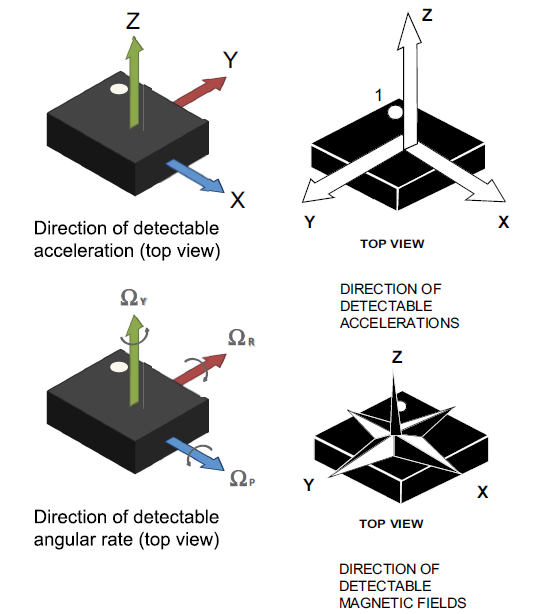
\includegraphics[scale=0.55]{figures/mems_axes.png}
			\caption{MEMS orientation}\label{fig:4a}
		\end{subfigure}
		\begin{subfigure}[H]{0.45\textwidth}
			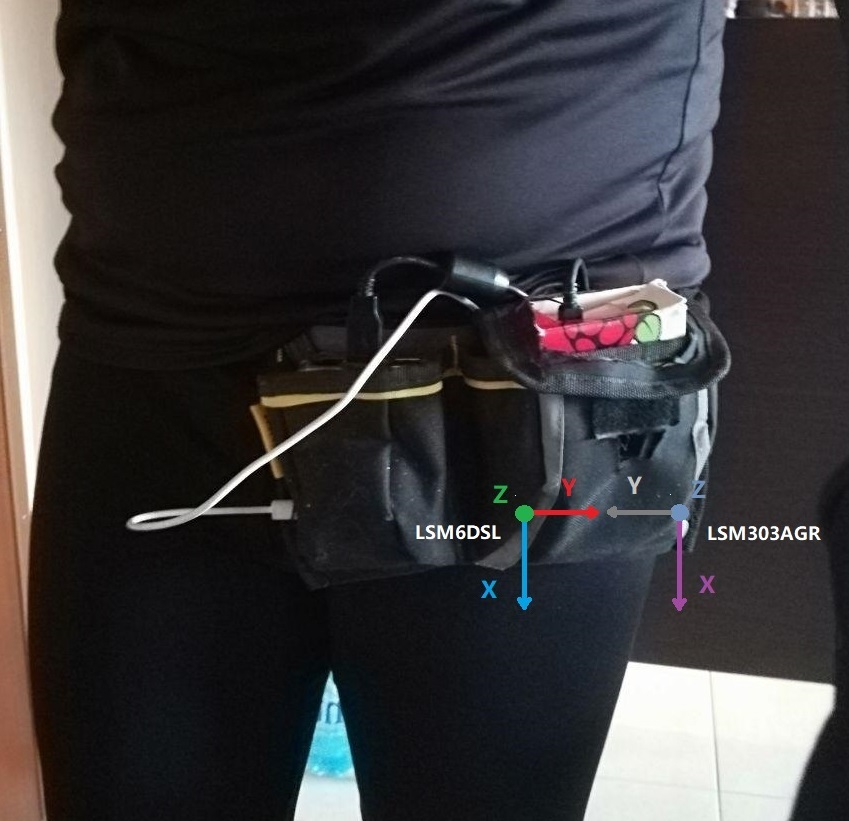
\includegraphics[scale=0.45]{figures/sensor_orientation.jpg}
			\caption{Axes w.r.t the body}\label{fig:4b}
		\end{subfigure}
	\end{figure} 
\end{center}
From MEMS positions it is possible to remark some considerations. Intuitively, it is expected to have some regular behaviour of the directional acceleration towards Z for walking and running activities:
\begin{figure}[H]
		\hfill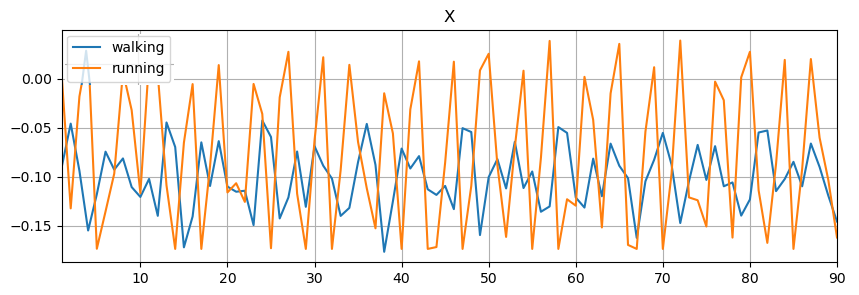
\includegraphics[scale=0.8]{figures/plot_ACC_LSM6DSL_DS_walking_running_X.png}\hspace*{\fill}
		\caption{LSM6DSL Accelerometer: running and walking}\label{fig:5}
		\centering
\end{figure}
This can be noticed from the "weird" behaviour in running trend with respect to walking, that on the other hand presents accentuated, but more distanced peaks (representing various steps).\newline
An easier comparison regards jumping and standing activities which instead, present more distinguishable regularities on X:
\begin{figure}[H]
		\hfill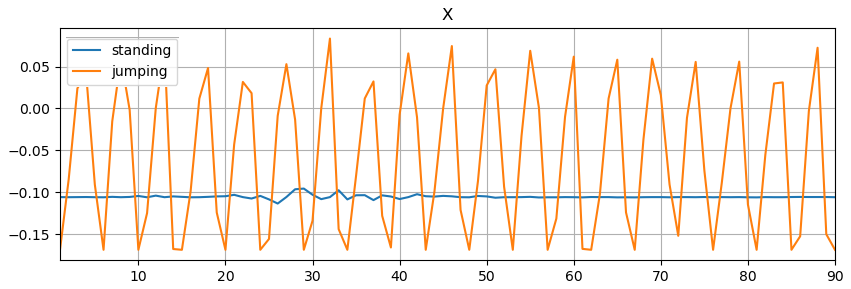
\includegraphics[scale=0.8]{figures/plot_ACC_LSM6DSL_DS_standing_jumping_X.png}\hspace*{\fill}
		\caption{LSM6DSL Accelerometer: jumping and standing}\label{fig:6}
		\centering
\end{figure} 
Same observation for supine, lying on side and sitting positions:
\begin{figure}[H]
	\hfill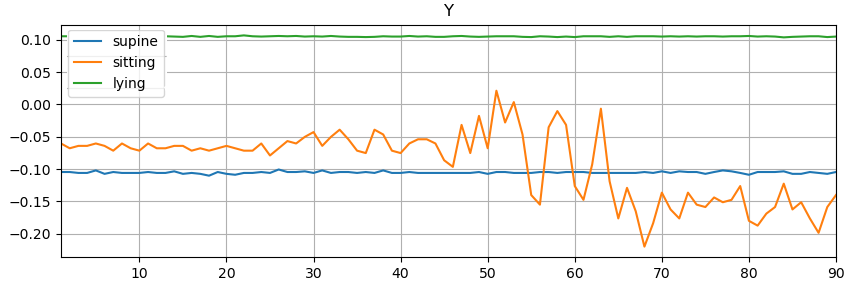
\includegraphics[scale=0.8]{figures/plot_ACC_LSM303AGR_DS_supine_sitting_lying_Y.png}\hspace*{\fill}
	\caption{LSM6DSL Accelerometer: sitting, supine, lying on side}\label{fig:7}
	\centering
\end{figure} 
This kind of analysis also helps to understand qualitatively the amount of efforts to dedicate in further session of data collection: if trends show evident patterns, it is reasonable to think that the AI algorithm needs not so many samples to learn them. Although other sensor trends do not show interesting regularities, from another perspective the importance of magnetometer in the pattern recognition is remarked by seeing directly to the distribution of a bunch of data points in a 3D scattering plot:
\begin{figure}[H]
	\hfill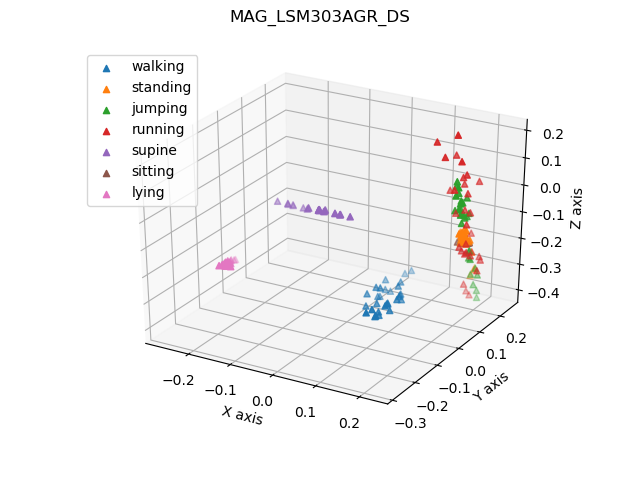
\includegraphics[scale=0.8]{figures/scatter3d_MAG_LSM303AGR_DS.png}\hspace*{\fill}
	\caption{LSM303AGR Magnetometer, Scattering Plot }\label{fig:8}
	\centering
\end{figure}
Most of the activity distributions appear to be distinguishable, but as it can be noticed, it is very difficult to discriminate between running and walking, or between standing and jumping in a certain range of values. The scattering plots of the LSM6DSL's accelerometer and gyroscope are even more confused and difficult to be analyzed:
\begin{center}
	\begin{figure}[H]
		\begin{subfigure}[H]{0.45\textwidth}
			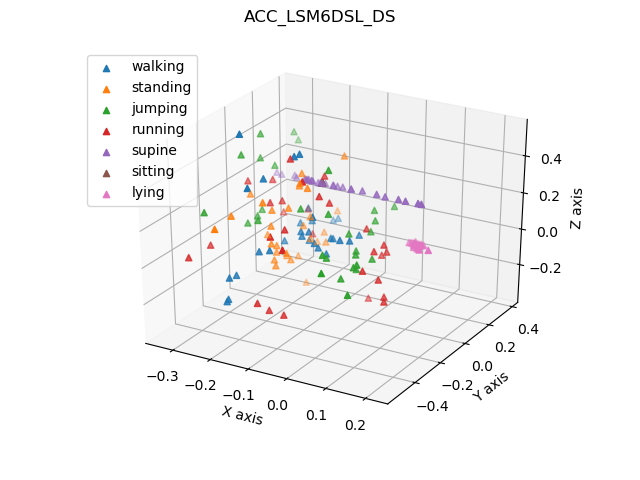
\includegraphics[scale=0.6]{figures/scatter3d_ACC_LSM6DSL_DS.png}
			\caption{LSM6DSL Accelerometer, Scattering Plot}\label{fig:8a}
		\end{subfigure}
		\begin{subfigure}[H]{0.45\textwidth}
			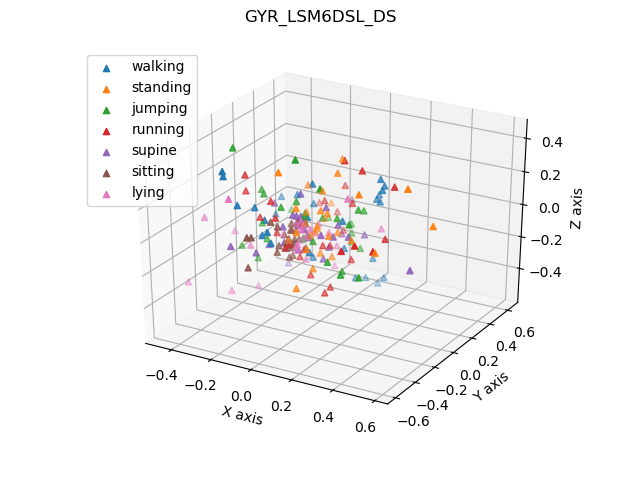
\includegraphics[scale=0.6]{figures/scatter3d_GYR_LSM6DSL_DS.png}
			\caption{LSM6DSL Gyroscope, Scattering Plot}\label{fig:8b}
		\end{subfigure}
	\end{figure} 
\end{center}
This is the reason why it is not so easy to write an algorithm to classify among 7 activities, by doing some statistical evaluation on samples in a very tight time window. This consideration does not preclude the possibility to use other machine learning techniques to solve this problem, but since such techniques have been frequently used in many similar research works, it has been decided to rely on neural networks this time.\newline
Focusing on the architecture, Recurrent Neural Networks (RNN) are an established standard in classification problems that involve time series. Besides this LSTM-based model  an alternative solution was developed originally, a simple Convolutional Neural Network (CNN) that  unfortunately did not provide satisfying results for this specific task. It will not be discussed in this report.\newline
The RNN solution consists in a single-cell LSTM architecture on top of a classifier, characterized by the following layers:


\begin{wrapfigure}{r}{0.4\textwidth}
	\hfill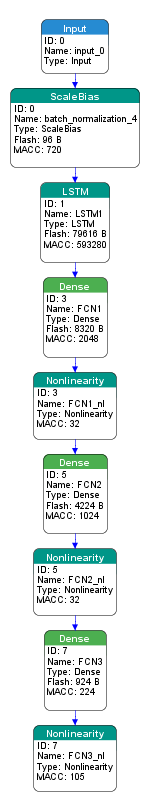
\includegraphics[width=0.2\textwidth]{figures/rnn.png}\hspace*{\fill}
	\caption{RNN model graph}\label{fig:9}
	\centering
	\vspace{-250pt}
\end{wrapfigure}
\noindent
\begin{itemize}
	\item \textbf{Batch Normalization}: to perform batch normalization of input data. Precisely, this layer performs \textit{standardization} of the input batch according to the following formulas:
	\[
		 y_{i} = \gamma \hat{x_{i}} + \beta \ \ \ \ \ \ \ \ 
		 \hat{x_{i}} = \frac{x_{i} - \mu_{B}}{\sqrt{\sigma_{B}^2 + \epsilon}}
	\]
	in which $x_{i}$ is a data point of the batch, $ \mu_{B} $ and $ \sigma_{B} $is the batch mean and variance respectively, whereas $ \gamma $ and $ \beta $ are paramters used to properly scale the normalization result, $ \epsilon $ at the end avoids zero-division. 
	\item \textbf{single LSTM} cell: characterized by 64 hidden nodes, with \textit{tanh} as activation function and \textit{sigmoid} as recurrent activation function. This part of the architecture is in charge of capturing time dependences in data sequence  
	\item \textbf{3 Fully-connected} layers: to classify features extracted by the LSTM cell, first layers (FCN1 and FCN2) composed of 32 neurons using a \textit{rectified-linear unit} as non-linear activation function and a last step of \textit{softmax} normalization . 
\end{itemize}
Here some implementation details:


\inputminted[framesep=1cm, firstline=52, lastline=68, bgcolor=whitesmoke, fontsize=\tiny]{python}{code/neural_network.py}
\newpage





\subsection{Network Training and Validation}
This step of the development process, starts from some preprocessing of the collected dataset files. Since each data gathering session is fully contained in a single csv file, it is required at first to group all the files associated to the same activity into a single one by using
\mintinline[bgcolor=whitesmoke]{python}{merge_session_files} function.\newline
After that, samples within each dataset are extracted into a dictionary to simplify possible use of preprocessing routines and prepared to be fed as input to the network for the training phase. Before proceding, it is important to remark that, in order to obtain reliable results the \textit{k-fold cross-validation} technique is used in the testing part, so different models of the same architecture are trained and the relative performances are then averaged, whereas at the end only the best accuracy and loss performance models are saved. 


\begin{wrapfigure}{r}{0.65\textwidth}
	\vspace{-20pt}
	\hfill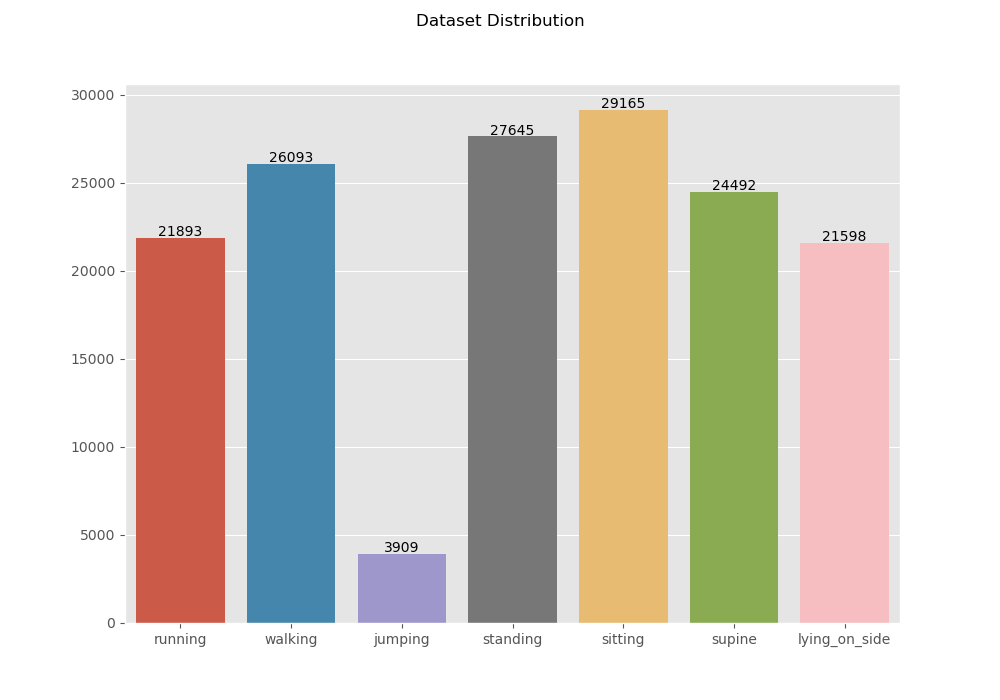
\includegraphics[width=0.65\textwidth]{figures/data_dist.png}\hspace*{\fill}
	\caption{Dataset Distribution}\label{fig:10}
	\centering
\end{wrapfigure}
A first look to the sample distribution per class, helps to understand that there is a risk of biasing the model performance on the activity with the largest number of samples. The dataset in fact, is strongly unbalanced due to the particular efforts required to collect data for some class with respect to the others (e.g: see jumping) and this factor represents a limitation in the final result.\newline
The number of models to train reflects the number of folds. The technique as well-known expects to leave one fold out and use the remaining ones for training, evaluating the generalization error on the excluded fold at the end. This procedure repeated for all the \textit{k} folds produces \textit{k} different models. \\
\par
\begin{wrapfigure}{l}{0.6\textwidth}
	\hfill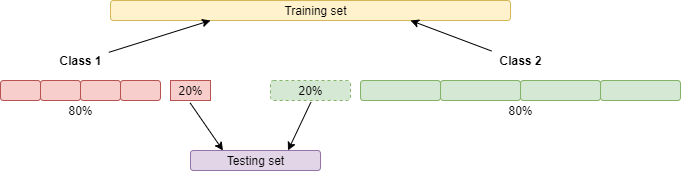
\includegraphics[width=0.55\textwidth]{figures/k_fold_part.png}\hspace*{\fill}
	\caption{Dataset partitioning}\label{fig:11}
	\centering
\end{wrapfigure}
In order to compensate this unbalanced distribution, fold partitioning is performed on each activity subset and the partitions then are all grouped together. \newline
One of the most important features of STM32Cube.AI, is that it allows to perform model testing directly on target either with randomly generated values or with a test set properly stored in a csv file. This possibility suggested to develop a function, \mintinline[bgcolor=whitesmoke]{python}{test_on_csv} in order to automatically create such file from the test partition of the dataset. \newline
As it can be noticed from the code, at a certain point preprocessed data are stacked in a categorical manner, this condition forces the algorithm to learn parameters per class, biasing the final result. As usual in such cases, an effective solution is to shuffle the entire dataset adding stochasticity in the way in which different data samples are fed to the network during training, this solution is implemented by the \mintinline[bgcolor=whitesmoke]{python}{shuffle_dataset} method.\newline
After data preprocessing, each network instance is trained sequentially for 60-80 epochs with 32 samples per batch, using RMSProp as optimization algorithm. Whatever solution is chosen the training settings are more or less the same except for the number of epochs which is tuned according to the adopted  solution.

\begin{table}[H]
	\begin{tabular}{||p{5cm}cc||}
		\hline
		Layer (type)      &           Output Shape        &      Params \T\B	\\
		\hline
		\hline
		BatchNormalization    &		  (None, 30, 12)       &     48          \T\B \\
		\hline
		LSTM1 (LSTM)          &       (None, 64)           &     19712     	 \T\B \\
		\hline
		FCN1 (Dense)          &       (None, 32)           &     2080       \T\B \\
		\hline
		FCN2 (Dense)          &       (None, 32)           &     1056      	\T\B \\
		\hline
		FCN3 (Dense)          &       (None, 7)            &     231       \T\B \\ 
		\hline
		\hline
		Total params:   &&										23,127\T  \\
		Trainable params:  && 	  								23,103\\
		Non-trainable params:  && 								24\B  \\
		\hline
		
	\end{tabular}
	\centering
	\caption{\label{tab:2}Recurrent Neural Network: Model Summary}
\end{table}
As the number of trainable parameters suggests, the network architecture is not so complex. Although this seems an advantage from computational perspective, it implies that the model is affected by a considerable amount of variance and it tends therefore to overfit and as experimented in final testing, regardless good validation results, the final application presents some slight performance degradation under changes in testing conditions.\newline
Hence different Dropout layers are added at training time and Early Stopping regularization technique has been adopted to prevent overfitting as well.

\begin{center}
	\begin{figure}[H]
		\begin{subfigure}[H]{0.45\textwidth}
			\hfill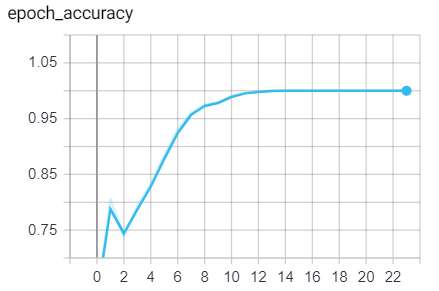
\includegraphics[scale=0.6]{figures/last_model_val_acc.png}\vspace*{\fill}
			\caption{Validation accuracy trend through epochs}\label{fig:8a}
		\end{subfigure}
		\begin{subfigure}[H]{0.45\textwidth}
			\hfill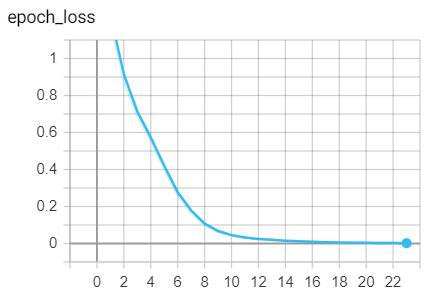
\includegraphics[scale=0.6]{figures/last_model_val_loss.png}\vspace*{\fill}
			\caption{Validation loss trend through epochs}\label{fig:8b}
		\end{subfigure}
	\end{figure} 
\end{center}
The training algorithm converges sharply after few epochs. From final validation considering all the trained models the average results appears better than expected, with:\\

\begin{wrapfigure}{r}{0.4\textwidth}
	\hfill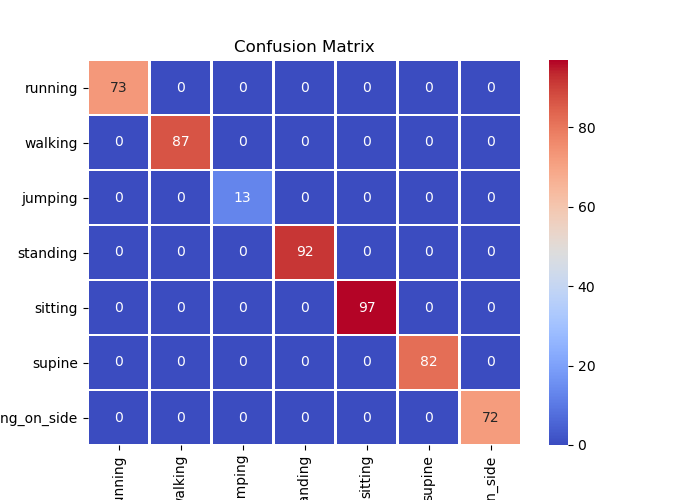
\includegraphics[width=0.6\textwidth]{figures/confmat_07-04-2020_202659.png}\hspace*{\fill}
	\caption{Confusion Matrix: Testing}\label{fig:9}
	\centering
	\vspace{-60pt}
\end{wrapfigure}
\noindent

\begin{itemize}
	\item \textbf{Average Validation Accuracy}: 0.9913
	\item \textbf{Average Validation Loss}: 0.0305
\end{itemize}
More optimistic results, instead come from the best trained model (fold 3) as shown in the confusion matrix (fig 17), that gives even a perfect prediction of all testing cases, the estimation however is even too optimistic as confirmed with other trained instances of the same architecture: some of them for example completely mispredicts jumping cases, so even if the chosen model is the best one, it should not be expected to have a perfect classifier at the end. Model ensemble techniques suggested by the literature are instead discouraged due to hardware constrains.

\subsection{Network Code Generation and on-target Testing}
STM32CubeMX, as mentioned in previous discussions, is in charge of generating the C-code from the Keras model, precisely an initialization of the network on which is possible to build a specific application, so what is really important in this step is that the developer is not worried about the embedded implementation of each network layer details.\newline
Before proceeding it is important to outline how the tool works in order to understand the way the network model is treated within the program environment, the AI plugin in fact, lives within STM32CubeMX that requires some preliminary configuration including the creation of a new project and some specification of the development board used. This step must be repeated at least once to generate all the required network files. STM32CubeAI offers a command-line interface that is exploited in this work to automatize validation and code generation

\begin{figure}[H]
	\hfill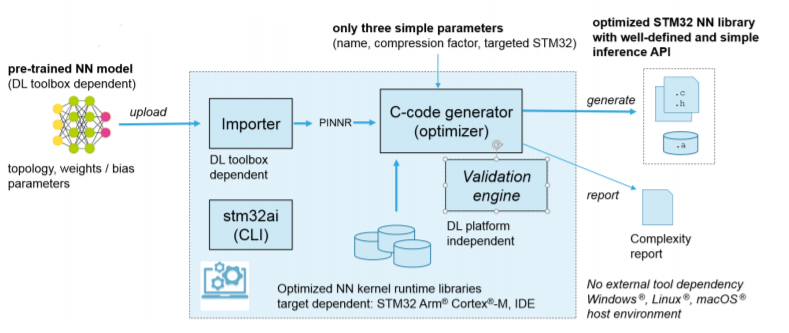
\includegraphics[width=0.8\textwidth]{figures/stm32cubeai_arch.png}\hspace*{\fill}
	\caption{X-CUBE AI Engine}
\end{figure}

After that, one of the h5 model files produced during training is imported and from the specific framework model, the tool builds a platform-independent representation (PINNR).\newline 
This new version of the model is used by the \textit{Validation Engine} to perform validation either locally or directly on the target board and the \textit{C-code generator} that generates the network code.\newline
So the first step, the model is imported into the project
Furthermore, it is important to highlight another interesting aspect that raises from a first analysis of the model summary created during training phase:




\subsection{Code Integration and Final Firmware Development}
 A challenging part in this work is represented by the integration  It includes the following folders:
\begin{itemize}
	\item \textbf{Drivers}: containing architecture-specific source files and in particular the implementation of network layer operations and non-linear activation functions
	\item \textbf{Inc}:  
\end{itemize} 



The main goal of this work is to show the resulting performance in terms of accuracy and response time required for the network to provide a single prediction


\section{Experimental evaluation}

\subsection{Experimental setup}

\subsection{Results}
\textbf{Please make sure you explicitely cite the tables.
\prettyref{tab:a_complex_table} shows a complex table.
Please also make sure you provide each table with an exhaustive caption.
Captions for tables must be placed before not after the tables.}



\begin{table}
\small
\begin{center}

\caption{Summary of the test scenarios.
$M_1\xrightarrow{\alpha}M_2$ means that an application mapping
is changed from $M_1$ to $M_2$ after application $\alpha$
has terminated.}
\begin{tabular}{l|lcc|L{2cm}l}
\cline{2-6}
& \multicolumn{3}{c|}{Description of the workload} & \multicolumn{2}{c}{Cores allocation}\\
\cline{2-6}
Name of scenario & Application & Threads & $\frac{Threads}{Cores}$ & HMP & HMP w/policy \\
\hline

\multirow{2}{*}{LITTLE 1} & ferret$\dagger$ & 1 & \multirow{2}{*}{1.00} & $0-3$ & $0$ \\
 & vips & 3 & & $0-3$ & $1-3 \xrightarrow{\dagger} 0-3$ \\
\hline
\multirow{2}{*}{LITTLE 2} & freqmine$\dagger$ & 2 & \multirow{2}{*}{1.25} & $0-3$ & $0-1$ \\
 & blackscholes & 3 &   & $0-3$ & $0-3 \xrightarrow{\dagger} 0-3$ \\
\hline
\multirow{2}{*}{LITTLE 3} & bodytrack$\dagger$ & 3 & \multirow{2}{*}{1.25} & $0-3$ & $0-1$ \\
 & facesim & 2 &  & $0-3$ & $0-3$ \\
\hline
\multirow{2}{*}{LITTLE 4} & facesim & 3 & \multirow{2}{*}{1.50} & $0-3$ & $0-1\xrightarrow{\dagger}0-3$ \\
 & blackscholes$\dagger$ & 3 &  & $0-3$ & $2-3$ \\
\hline
\hline


\multirow{2}{*}{big 1} & vips & 3 & \multirow{2}{*}{1.00} & $4-7$ & $4-5 \xrightarrow{\dagger} 4-7$ \\
 & ferret$\dagger$ & 1 & & $4-7$ & $6-7$ \\
\hline
\multirow{2}{*}{big 2} & freqmine$\dagger$ & 2 & \multirow{2}{*}{1.25} & $4-7$ & $4-5$ \\
 & blackscholes & 3 &   & $4-7$ & $6-7 \xrightarrow{\dagger} 4-7$ \\
\hline
\multirow{2}{*}{big 3} & facesim & 2 & \multirow{2}{*}{1.25} & $4-7$ & $4-5$ \\
 & bodytrack & 3 &  & $4-7$ & $4-7$ \\
\hline
\multirow{2}{*}{big 4} & facesim & 3 & \multirow{2}{*}{1.50} & $4-7$ & $4-5\xrightarrow{\dagger}4-7$ \\
 & blackscholes$\dagger$ & 3 &  & $4-7$ & $4-7$ \\
\hline

\end{tabular}
  \label{tab:a_complex_table}
\end{center}
\end{table}

\section{Conclusions and Future Works}

